\documentclass[../main.tex]{subfiles}
\graphicspath{
    {"../img/"}
    {"img/"}
}
\begin{document}

\begin{figure}[h]
    \centering
    \includegraphics[width=0.6\textwidth]{fig_14}
    \caption{Inne podejście: iterujemy funkcję na jej wyniku}
\end{figure}

\begin{definicja}
    Niech $L: V\to W, L$ - liniowe, $(V,||.||_v),(W,||.||_w)$ - unormowane.
    Mówimy, że $L$ jest ograniczone, jeżeli
    \[
        \underset{A>0}{\exists}\quad\underset{x\in V}{\forall} ||L(x)||_w \leq A||x||_v.
    \]
\end{definicja}

\begin{przyklad}


$\text{dla }
\left [ \begin{matrix}
x\\
y\\
\end{matrix}\right ] \in \mathbb{R}^2, f(x,y) : \mathbb{R}^2 \to \mathbb{R}^2$\\
\[
    \underset{A}{\exists}\quad \forall
    \left [ \begin{matrix}
    x\\
    y\\
     \end{matrix}\right ] \in \mathbb{R}^2,\quad \left\Vert \left [ \begin{matrix}
    \frac{1}{2} &0\\
    0 &\frac{1}{2}\\
     \end{matrix}\right ]
    \left [ \begin{matrix}
    x\\
    y\\ \end{matrix}\right ] \right\Vert
    \leq A \left\Vert \left [ \begin{matrix}
    x\\
    y\\ \end{matrix}\right ]
    \right\Vert
\]

ale
\[
    \forall \left [ \begin{matrix}
    x\\
    y\\
     \end{matrix}\right ] \in \mathbb{R}^2, \Bigg | \Bigg |
    \left [ \begin{matrix}
    \frac{1}{2} &0\\
    0 & \frac{1}{2}\\
     \end{matrix}\right ]
    \left [ \begin{matrix} x\\
    y\\ \end{matrix}\right ]
    \Bigg | \Bigg | < \frac{1}{2} \Bigg | \Bigg |  \left [ \begin{matrix}
    x\\
    y\\ \end{matrix}\right ] \Bigg | \Bigg|
\]
\end{przyklad}

\begin{tw}
    ($L$ - ograniczone) $\iff$ ($L$ - ciągłe)
\end{tw}

\begin{proof}
    $\impliedby$\\
    Wiemy, że
\[
    \underset{\varepsilon > 0}{\forall}, \underset{\delta}{\exists}, \underset{x,x'\in V}{\forall},\quad ||x-x'||_v < \delta \implies ||L(x) - L(x')||(*)< \varepsilon
,\]
chcemy pokazać, że:
\[
    \underset{A>0}{\exists}.\underset{x,x'\in V}{\forall}\quad ||L(x-x')|| \leq A||x-x'||,
\]
zatem wiemy, że para $(\varepsilon, \delta)$ spełniająca warunek $(*)$ istnieje.\\
Ale
    \[
        ||L(x-x')|| = \underbrace{\Bigg |\Bigg |L\left ( \frac{x-x'}{||x-x'||}\right ) \frac{\delta}{2}\Bigg |\Bigg | \frac{||x-x'|| 2}{\delta}}_{\text{własność liniowości i normy}} \leq \varepsilon \frac{||x-x'|| 2}{\delta}
    \]
Co wiemy o $\left\Vert \frac{x-x'}{||x-x'||} \frac{\delta}{2} \right\Vert_v < \delta?$

$$\underset{x,x'\in V}{\forall}||L(x-x')||_w \leq \frac{2 \varepsilon}{\delta} ||x-x'||_v$$
Szukane $A=\frac{2\varepsilon}{\delta}$ istnieje!
\end{proof}

\begin{proof}
    $\implies$\\
Wiemy, że
\begin{equation}\label{eq:d1}
    \underset{A}{\exists}\quad \underset{x,x'\in V}{\forall}\quad \left\Vert L(x-x')\right\Vert \leq A\left\Vert x-x' \right\Vert
\end{equation}

Chcemy pokazać, że jeżeli $x_n\to x_0$, to $L(x_n)\to L(x_0)$, ale
\[
    0 \leq ||L(x_n)-L(x_0)||_w = ||L(x_n-x_0)||_w \leq A||x_n-x_0||(\text{ bo (\ref{eq:d1})})
\]
\[
    0\leq ||L(x_n) - L(x_0)||_w \leq A||x_n - x_0||(\text{ wszystko dąży do 0)}
\]
\end{proof}

\begin{definicja}
    Wielkość
    \[
        \underset{A}{inf} \{\underset{x\in V}{\forall}||L(x)||_w \leq A||x||_v\}
    \]
    nazywamy normą odwzorowania $L$ i oznaczamy $A\overset{\text{ozn}}{=}||L||$.
\end{definicja}
\begin{definicja}
    Niech $U\subset \mathbb{R}^m$ - jest zbiorem wypukłym, jeżeli
    \[
        \underset{a,b\in U}{\forall}\quad [a,b]\overset{\text{def}}{=} \left \{ a(1-t)+bt, t\in[0,1] \right \} \subset U
    \]
\end{definicja}
\begin{figure}
    \centering
    \includegraphics[width=0.6\textwidth]{fig_15}
    \caption{zbiór wklęsły}
\end{figure}
\begin{figure}
    \centering
    \includegraphics[width=0.6\textwidth]{fig_16}
    \caption{zbiór wypukły}
\end{figure}

\pagebreak
\begin{stw}
    Niech $f: U\subset \mathbb{R}^m \to \mathbb{R}^n, U$ - wypukłe,
    \[
        \underset{M}{\exists}\quad \underset{x\in U}{\forall}||f'(x)||\leq M
    ,\]
to
    \[
        \underset{a,b\in U}{\forall}||f(b)-f(a)||_n \leq M||b-a||_m
    \] \begin{tiny}(jakiekolwiek skojarzenia z Twierdzeniem Lagrange zupełnie przypadkowe *wink* *wink*)\end{tiny}
\end{stw}

\begin{proof}

niech $\gamma (t) = a(1-t) + bt, t\in [0,1], \quad g(t) = f(\gamma (t)),g: \mathbb{R}^1 \to \mathbb{R}^n$,
czyli
\[
    g(t) = \left [ \begin{matrix}
    g_1(t)\\
    g_2(t)\\
    \vdots\\
    g_n(t)\\ \end{matrix}\right ]
,\]
zatem
    \begin{align*}
        \left \Vert g(1)-g(0)\right \Vert &= \left \Vert \left [ \begin{matrix}
    g_1(1) - g_1(0)\\
    g_2(1) - g_2(0)\\
    \vdots\\
    g_n(1) - g_n(0)\\ \end{matrix}\right ] \right \Vert \overset{\text{Tw. Lagrange!}}{=}\\
        &=\left\Vert \underset{0<c_i<1}{\left [ \begin{matrix}
    g_1'(c_1)(1-0)\\
    g_2'(c_2)(1-0)\\
    \vdots\\
        g_n'(c_n)(1-0)\\ \end{matrix}\right ]}\right\Vert \leq \left\Vert \left [ \begin{matrix}
    g_1'(c_1)\\
    g_2'(c_2)\\
    \vdots\\
    g_n'(c_n)\\ \end{matrix}\right ] \right\Vert \left\Vert 1 - 0 \right\Vert
    \end{align*}

\[
    \text{Ale } g'(t) = f'(\gamma(t))\gamma'(t) \to \left\Vert g'(t)\right\Vert = \left\Vert f'(\gamma(t))(b-a)\right\Vert \leq \left\Vert f'(\gamma(t))\right\Vert \left\Vert b-a \right\Vert \underset{\text{z zał. stw.}}{\leq} M
\]
\[
    \text{Czyli }\underset{t\in[0,1]}{\forall}\left\Vert g'(t) \right\Vert \leq M\left\Vert b-a \right\Vert \implies \left\Vert f(b) - f(a) \right\Vert \leq M \left\Vert b - a \right\Vert
\]
\end{proof}


\begin{definicja}
Niech $X$ - unormowana: $P: X\to X, P$ - ciągła na $X$.\\
Interesuje nas zbieżność ciągów typu $\{x_0, P(x_0), P(P(x_0)),\dots \}, x_0\in X$\\
    $\tilde x \in X$ nazywamy punktem stałym, jeżeli $P(\tilde x) = \tilde x$
\end{definicja}

\begin{figure}[h]
    \centering
    \includegraphics[width=0.5\textwidth]{fig_17}
\end{figure}

\begin{tw}
Jeżeli ciąg $\{x_0, P(x_0), \dots \} $ - zbieżny i $P$ - ciągłe, to jest on zbieżny do punktu stałego.
\end{tw}

\begin{proof}

Niech $x_n = P^{(n)} (x_0)$. Wiemy, że $x_n$ - zbieżny, oznaczmy granicę tego ciągu przez $\tilde x$.
Mamy:
\begin{equation}\label{eq:d2}
    \underset{\varepsilon_1 > 0}{\forall}\quad \underset{N_1}{\exists}\quad \underset{n>N_1}{\forall}\quad d(x_n,\tilde x) < \varepsilon_1
\end{equation}
\begin{equation}\label{eq:d3}
    \underset{\varepsilon_2>0}{\forall}\quad \underset{N_2}{\exists}\quad \underset{n>N_2}{\forall}\quad d(x_{n-1},\tilde x) < \varepsilon_2
\end{equation}
$P$ - ciągłe, czyli
    \[
        \underset{\varepsilon>0}{\forall}\quad \underset{\delta}{\exists}\quad \underset{x'}{\forall}:\quad d(x,x')<\delta \implies d(P(x),P(x'))<\varepsilon \text{, bo (\ref{eq:d2})}
    \]
Chcemy pokazać, że
\begin{equation}\label{eq:d4}
    \underset{\varepsilon>0}{\forall}\quad d(\tilde x,P(\tilde x))<\varepsilon
\end{equation}
Ale
\begin{equation}\label{eq:ep}
    d(\tilde x, P(\tilde x)) \leq d(\tilde x,x_n) + d(x_n, P(\tilde x)) = d(\tilde x, x_n) + d(P(x_{n-1}),P(\tilde x)) < \varepsilon + \varepsilon = 2 \varepsilon
\end{equation}
\begin{equation}
    \text{Ale z (\ref{eq:d2}) wynika, że }
    \underset{\varepsilon>0}{\forall}\quad \underset{\delta}{\exists}\quad d(x_{n-1},\tilde x) < \delta \implies d(P(x_{n-1}),P(\tilde x)) < \varepsilon
\end{equation}
Zatem znając $\varepsilon$ z (\ref{eq:d4}) przyjmujemy $\varepsilon_1 = \varepsilon$, oprócz tego znajdujemy $\delta$ przyjmując $\varepsilon_1 = \varepsilon$, a potem położymy $\varepsilon_2 = \delta$ z (\ref{eq:d3}) i dzięki temu mamy (\ref{eq:ep})
\end{proof}


\begin{definicja}
    Niech $X$ - przestrzeń metryczna, odwzorowanie $P: X\to X$ nazywamy zwężającym, jeżeli:
    \begin{equation}\label{eq:zwezajace}
        \underset{q\in [0,1[}{\exists}\quad \underset{x,y\in X}{\forall} d(P(x),P(y)) \leq q d(x,y)
    \end{equation}
\end{definicja}

\pagebreak
\begin{tw}
    (Zasada Banacha o lustrach)\\
    Jeżeli $P: X \to X, P$ - zwężające, to
    \begin{align}\label{eq:banach}
        &\text{1. } \underset{x_0 \in X}{\forall}\quad \{x_0,P(x_0),P(P(x_0)),\dots\}) \text{ - Zbieżny do punktu stałego } \tilde x\\
        &\text{2. Istnieje tylko jedno }\tilde x\\
        &\text{3. } \underset{m}{\forall}\quad d(x_m,\tilde x) < \frac{q^m}{1-q} d(x_1, x_0)
    \end{align}
\end{tw}


\begin{przyklad}
    \textbf{(Uwaga)}\\
($P$ - nie musi być ciągłe) - potem się okaże, że ciągłość gdzieś tutaj siedzi \textit{implicite}\\
\noindent- lustra w łazience koło sali 1.01 $\rightarrow$ można stanąć tak, że jedno jest przed tobą a drugie za tobą i wtedy te odbicia się ciągną w nieskończoność i zbiegają do punktu\\
- telewizor + kamera która go nagrywa a on wyświetla ten obraz\\
- mapa położona na podłodze zawiera dokładnie jeden punkt, który się pokrywa z miejscem na którym leży
\end{przyklad}
\begin{proof}
ad. 2\\
Załóżmy, że
    \[
        \underset{\tilde x_1, \tilde x}{\exists} P(\tilde x_1) = \tilde x_1, P(\tilde x_2) = \tilde x_2, \tilde x_1 \neq \tilde x_2
    \]
Wtedy
    \[
        d(\tilde x_1, \tilde x_2) = d(P(\tilde x_1),P(\tilde x_2)) < qd(\tilde x_1, \tilde x_2)
    \]
Dalej:
    \[
        d(\tilde x_1, \tilde x_2) \leq q d(\tilde x_1, \tilde x_2)\text{, ale }0\leq q \leq 1,\tilde x_1 \neq \tilde x_2 \implies \text{ sprzeczność! }
    \]
\end{proof}
\begin{proof}
\begin{obserwacja}


\begin{align*}
    d(x_{n+1},x_n) &= d(P(x_n),P(x_{n-1})) \leq qd(x_n, x_{n-1}) = qd(P(x_{n-1}),P(x_{n-2})) \leq\\
    &\leq q^2 d(x_{n-1},x_{n-2}) \leq q^n d(x_1,x_0)
.\end{align*}
Co, jeżeli zamiast $n+1$ weźmiemy $n+m$?
\begin{align*}
    d(x_{n+m},x_n) &\leq d(x_{n+m},x_{n+m+1}) + d(x_{n+m-1},x_n) \leq\\
    &\leq d(x_{n+m},x_{n+m-1}) + d(x_{n+m-1},x_{n+m-2}) + d(x_{n+m-2},x_n)\leq\\
    &\leq \dots\leq d(x_{n+m},x_{n+m-1}+ \dots+d(x_{n+1},x_n)\leq \\
    &\leq (q^{n+m-1} + \dots + q^{n+2} + q^{n+1} + q^n)d(x_1,x_0) \leq\\
    &\leq q^n \left ( \frac{1-q^n}{1-q} \right ) d(x_1,x_0) \underset{0\leq q<1}{\leq} \frac{q^n}{1-q} d(x_1,x_0)
.\end{align*}
Czyli $d(x_{n+m},x_n) \leq \frac{q^n}{1-q} d(x_1,x_0)$\\
\end{obserwacja}

Skoro $X$ - zupełna, to jeżeli $x_n$ - Cauchy, to znaczy, że jest zbieżny w $X$.
Czyli czy
$$\underset{\varepsilon>0}{\forall}\underset{N}{\exists}\underset{n,m>N}{\forall}\quad d(x_n,x_m) <\varepsilon ?$$

Załóżmy, że $m>n$ i $m=n+k$. Wtedy
$$\underset{\varepsilon>0}{\forall}\underset{N}{\exists}\underset{n>N}{\forall}\quad d(x_n,x_{n+k}) < \varepsilon? \text{ TAK!}$$
Dla $N$ takiego, że $\frac{q^N}{1-q} d(x_1,x_0) < \varepsilon$. Stąd wiadomo, że $x_n$ - Cauchy, czyli jest zbieżny. $x_n \to \tilde x$, zatem jeżeli $d(x_{n+m},x_n)\leq \frac{q^n}{1-q} d(x_1,x_0) \rightarrow d(\tilde x,x_n) \leq \frac{q^n}{1-q} d(x_1,x_0).$
\end{proof}
\end{document}
